\section{Differential Cross-Section}
\label{sec:differential cross-section}

The analysis method is very similar to the previously published one \cite{totem-1km}. The only important difference stems from using different RPs for the measurement: unit 210-fr instead of 220-nr as in \cite{totem-1km} which was not anymore equipped with sensors. Due to the optics and beam parameters the unit 210-fr has worse low-$|t|$ acceptance, further deteriorated by the tilt of the unit. Consequently, in order to maintain the low-$|t|$ reach essential for this study, the main analysis (denoted ``2RP'') only uses the 220-fr units. Since the abandon of the 210-nr unit may, in principle, result in worse resolution and background suppression, for control reasons, the traditional analysis with all units (denoted ``4RP'') was pursued, too. In Section~\ref{sec:cross checks} the ``2RP'' and ``4RP'' will be compared showing a very good match. In what follows, the ``2RP'' analysis will be described unless stated otherwise.

\TODO{mention that normalisation from a different dataset?}

Section~\ref{sec:event analysis} covers all aspects related to the reconstruction of a single event. Section~\ref{sec:diff cs} describes the steps of transforming a raw $t$-distribution into the differential cross-section. The $t$-distributions are analysed separately for each LHC fill and each diagonal. After comparison (Section~\ref{sec:cross checks}) they are finally merged (Section~\ref{sec:final data merging}).

%----------------------------------------------------------------------------------------------------
\subsection{Event Analysis}
\label{sec:event analysis}

The event kinematics are determined from the coordinates of track hits in the RPs after proper alignment (see Sec.~\ref{sec:alignment}) using the LHC optics (see Sec.~\ref{sec:optics}).

%------------------------------

\subsubsection{Kinematics Reconstruction}
\label{sec:kinematics}

For each event candidate the scattering angles of both protons (one per arm) are first estimated separately. In the ``2RP'' analysis, these formulae are used:
\begin{equation}
\label{eq:kin 1a}
	\theta^{*\rm L,R}_x = {x\over L_x}\ ,\quad \theta^{*\rm L,R}_y = {y\over L_y}
\end{equation}
where L and R refer to the left and right arm, respectively, and $x$ and $y$ stand for the proton position in the 220-fr unit. This one-arm reconstruction is used for tagging elastic events, where the left and right arm protons are compared.

Once a proton pair has been selected, both arms are used to reconstruct the kinematics of the event
\begin{equation}
\label{eq:kin 2a}
		\theta_x^* = {1\over 2} \left( \theta^{*\rm L}_x + \theta^{*\rm R}_x \right)\ ,\qquad
		\theta_y^* = {1\over 2} \left( \theta^{*\rm L}_y + \theta^{*\rm R}_y \right)\ .
\end{equation}
Thanks to the left-right symmetry of the optics and elastic events, this combination leads to cancellation of the vertex terms (cf.~Eq.~(\ref{eq:prot trans})) and thus to improvement of the angular resolution (see Section \ref{sec:resolution}).

Eventually, the scattering angle, $\theta^*$, and the four-momentum transfer squared, $t$, are calculated:

\begin{equation}
\label{eq:th t}
\theta^* = \sqrt{{\theta_x^*}^2 + {\theta_y^*}^2}\ ,\qquad t = - p^2 ({\theta_x^*}^2 + {\theta_y^*}^2)\ ,
\end{equation}
where $p$ denotes the beam momentum.

In the ``4RP'' analysis, the same reconstruction as in \cite{totem-1km} is used which allows for stronger elastic-selection cuts, see Section~\ref{sec:tagging}.



%------------------------------

\subsubsection{Alignment}
\label{sec:alignment}

TOTEM's usual three-stage procedure (Section 3.4 in~\cite{totem-ijmp}) for correcting the detector positions and rotation angles has been applied: a beam-based alignment prior to the run followed by two offline methods. First, track-based alignment for relative positions among RPs, and second, alignment with elastic events for absolute position with respect to the beam -- repeated in 20 minutes time intervals to check for possible beam movements.

Exploiting all the methods, the alignment uncertainties have been estimated to $25\un{\mu m}$ (horizontal shift), $100\un{\mu m}$ (vertical shift) and $2\un{m rad}$ (rotation about the beam axis). Propagating them through Eq.~(\ref{eq:kin 2a}) to reconstructed scattering angles yields $0.50\un{\mu rad}$ ($0.35\un{\mu rad}$) for the horizontal (vertical) angle. RP rotations induce a bias in the reconstructed scattering angles:
\begin{equation}
\label{eq:alig rot bias}
	\theta_x^* \rightarrow \theta_x^* + c \theta_y^*\ ,\quad
	\theta_y^* \rightarrow \theta_y^* + d \theta_x^*\ ,
\end{equation}
where the proportionality constants $c$ and $d$ have a mean of 0 and a standard deviations of $0.013$ and $3.9\cdot10^{-4}$, respectively.

\TODO{Mention that y misalignment is mostly top-bottom correlated? Mention the uncorrelated contribution?}



%------------------------------

\subsubsection{Optics}
\label{sec:optics}

It is crucial to know with high precision the LHC beam optics between IP5 and the RPs, i.e. the behaviour of the spectrometer composed of the various magnetic elements. The optics calibration has been applied as described in~\cite{totem-optics}. This method uses RP observables to determine fine corrections to the optical functions presented in Eq.~(\ref{eq:prot trans}).

In each arm, the residual errors induce a bias in the reconstructed scattering angles:
\begin{equation}
\label{eq:opt bias}
	\theta_x^* \rightarrow (1 + b_x)\, \theta_x^*\ ,\qquad
	\theta_y^* \rightarrow (1 + b_y)\, \theta_y^*\ .
\end{equation}
the biases $b_x$ and $b_y$ have uncertainties of $0.17\un{\%}$ and $0.15\un{\%}$, respectively, and a correlation factor of $-0.90$. \TODO{true?:} These estimates include the effects of magnet harmonics.

To evaluate the impact on the $t$-distribution, it is convenient to decompose the correlated biases $b_x$ and $b_y$ into eigenvectors of the covariance matrix:
\begin{equation}
\label{eq:opt bias modes}
\begin{pmatrix} b_x^{\rm L}\cr b_y^{\rm L} \cr b_x^{\rm R}\cr b_y^{\rm R} \end{pmatrix} =
	   \eta_1 \underbrace{\begin{pmatrix} -1.608\cdot10^{-3}\cr +1.473\cdot10^{-3}\cr -1.630\cdot10^{-3}\cr +1.477\cdot10^{-3} \end{pmatrix}}_{\rm mode\ 1}
  \ +\ \eta_2 \underbrace{\begin{pmatrix} -5.157\cdot10^{-4}\cr +2.541\cdot10^{-5}\cr +5.566\cdot10^{-4}\cr +2.746\cdot10^{-5} \end{pmatrix}}_{\rm mode\ 2}
  \ +\ \eta_3 \underbrace{\begin{pmatrix} +3.617\cdot10^{-4}\cr +3.625\cdot10^{-4}\cr +3.006\cdot10^{-4}\cr +3.641\cdot10^{-4} \end{pmatrix}}_{\rm mode\ 3}
\end{equation}
normalised such that the factors $\eta_{1,2,3}$ have unit variance. The fourth eigenmode has a negligible contribution and therefore is not explicitly mentioned.



%------------------------------

\subsubsection{Resolution}
\label{sec:resolution}

TODO



%----------------------------------------------------------------------------------------------------
\subsection{Differential Cross-Section Reconstruction}
\label{sec:diff cs}

For a given $t$ bin, the differential cross-section is evaluated by selecting and counting elastic events:
\begin{equation}
{\d\sigma\over \d t}(\hbox{bin}) =
	\mathcal{N}\, \mathcal{U}({\rm bin})\, \mathcal{B}\, {1\over \Delta t}
	\sum\limits_{t\, \in\, {\rm bin}} \mathcal{A}(\theta^*, \theta_y^*)\ \mathcal{E}(\theta_y^*)
	\ ,
\end{equation}
where $\Delta t$ is the width of the bin, $\mathcal{N}$ is a normalisation factor and the other symbols stand for various correction factors: $\mathcal{U}$ for unfolding of resolution effects, $\mathcal{B}$ for background subtraction, $\mathcal{A}$ for acceptance correction and $\mathcal{E}$ for detection and reconstruction efficiency.



%-------------------------

\subsubsection{Event Tagging}
\label{sec:tagging}


\begin{table}
\caption{The elastic selection cuts. The superscripts R and L refer to the right and left arm. The right-most column gives a typical RMS of the cut distribution.
}
\label{tab:cuts}
\begin{center}
%\vskip-3mm
\begin{tabular}{ccc}\hline
number & cut & RMS ($\equiv 1\sigma$)\cr\hline
1 & $\theta_x^{*\rm R} - \theta_x^{*\rm L}$				& $14\un{\mu rad}$	\cr
2 & $\theta_y^{*\rm R} - \theta_y^{*\rm L}$				& $0.38\un{\mu rad}$	\cr\hline
\end{tabular}
\end{center}
\end{table}

For the ``2RP'' analysis one may apply the cuts requiring the reconstructed-track collinearity between the left and right arm, see Table~\ref{tab:cuts}. The correlation plots corresponding to these cuts are shown in Figure~\ref{fig:cuts}.

\begin{figure}
\begin{center}
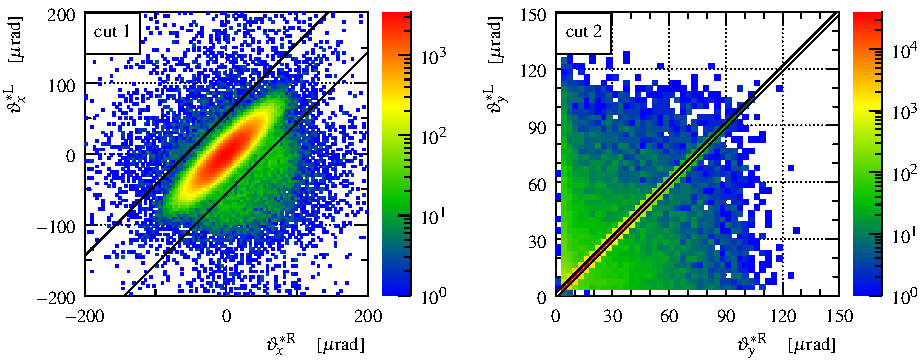
\includegraphics{fig/cut_example.pdf}
\caption$ of the elastic events, the cut threshold is set to $4\un{\sigma}$.

The tagging efficiency has been studied by applying the cuts also at the $5\un{\sigma}$-level. This selection has yielded about $0.1\un{\%}$ more events in every $|t|$-bin. This kind of inefficiency only contributes to a global scale factor, which is irrelevant for this analysis because the normalisation is taken from a different data set (cf. Section~\ref{sec:normalisation}).

In the ``4RP'' analysis, thanks to the additional information from the 210-fr units, more cuts can be applied (cf.~Table~2 in~\cite{epl101-el}). In particular the left-right comparison of the reconstructed horizontal vertex position, $x^*$, and vertical position-angle correlation in each arm. Furthermore, since the single-arm reconstruction can disentangle the contributions from $x^*$ and $\theta^*_x$, the angular resolution is better compared to the ``2RP'' analysis and consequently cut 1 becomes more stringent.

\TODO{which xi values are accepted}




%-------------------------

\subsubsection{Background}
\label{sec:background}

As the RPs were very close to the beam, one may expect an enhanced background from coincidence of beam halo protons hitting detectors in the two arms. Other background sources (pertinent to any elastic analysis) are: central diffraction and pile-up of two single diffraction events.

The background rate (i.e.~impurity of the elastic tagging) is estimated in two steps, both based on distributions of discriminators from Table~\ref{tab:cuts} plotted in various situations, see an example in Figure~\ref{fig:tag bckg integ}. In the first step, diagonal data are studied under several cut combinations. While the central part (signal) remains essentially constant, the tails (background) are strongly suppressed when the number of cuts is increased. In the second step, the background distribution is interpolated from the tails into the signal region. The form of the interpolation is inferred from non-diagonal RP track configurations (\textit{45 bottom -- 56 bottom} or \textit{45 top -- 56 top}), artificially treated like diagonal signatures by inverting the $y$ coordinate sign in the arm 45. These non-diagonal configurations cannot contain any elastic signal and hence consist purely of background which is expected to be similar in the diagonal and non-diagonal configurations. This expectation is supported by the agreement of the tails of the blue solid and dashed curves in the figure. Since the non-diagonal distributions are flat, the comparison of the signal-peak size to the amount of interpolated background yields the estimate $1 - \mathcal{B} = \mathcal{O}(10^{-3})$.

\begin{figure}
\begin{center}
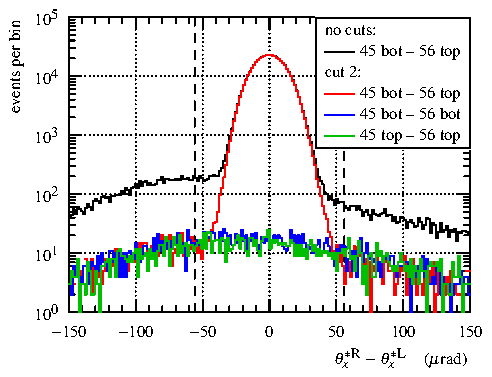
\includegraphics{fig/cut_dist_antidgn_cmp.pdf}
\caption{%
Distributions of discriminator 1, i.e. the difference between the horizontal scattering angle reconstructed from the right and the left arm. Data from LHC fill 5314. Black and red curves: data from diagonal 45 bottom -- 56 top, the different colours correspond to various combinations of the selection cuts (see numbering in Table~\ref{tab:cuts}). Blue and green curves: data from anti-diagonal RP configurations, obtained by inverting track $y$ coordinate in the left arm. The vertical dashed lines represent the boundaries of the signal region ($\pm 4\un{\sigma}$).
}
\label{fig:tag bckg integ}
\end{center}
\end{figure}

\TODO{describe} Figure~\ref{fig:tag bckg dist}. Apply some correction?

\begin{figure}
\begin{center}
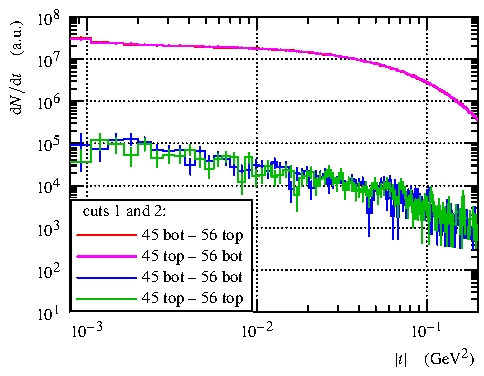
\includegraphics{fig/t_dist_antidgn_cmp.pdf}
\caption{%
$|t|$ distributions from different diagonal and anti-diagonal configurations, after all cuts and acceptance correction. Data from LHC fill 5314.
}
\label{fig:tag bckg dist}
\end{center}
\end{figure}

%-------------------------

\subsubsection{Acceptance Correction}
\label{sec:acc corr}

TODO

%-------------------------

\subsubsection{Inefficiency Corrections}
\label{sec:ineff corr}

TODO

%-------------------------

\subsubsection{Unfolding of Resolution Effects}
\label{sec:unfolding}

TODO

%-------------------------

\subsubsection{Normalisation}
\label{sec:normalisation}

TODO

%-------------------------

\subsubsection{Binning}
\label{sec:binning}

TODO

%-------------------------

\subsubsection{Systematic Uncertainties}
\label{sec:systematics}

TODO

%----------------------------------------------------------------------------------------------------

\subsection{Systematic Cross-Checks}
\label{sec:cross checks}

TODO


 %----------------------------------------------------------------------------------------------------
\subsection{Final Data Merging}
\label{sec:final data merging}

TODO
